\documentclass[11pt,
			   %10pt, 
               %hyperref={colorlinks},
               aspectratio=169,
               hyperref={colorlinks}
               ]{beamer}
\usetheme{Singapore}
\usecolortheme[snowy, cautious]{owl}

\usepackage[utf8]{inputenc}
\usepackage[T1]{fontenc}
\usepackage[american]{babel}
\usepackage{graphicx}
\usepackage{hyperref}
\hypersetup{
    colorlinks=true,
    urlcolor=magenta,
    linkcolor=violet}

\usepackage[natbib=true,style=authoryear,backend=bibtex,useprefix=true]{biblatex}

%\setbeamercolor*{bibliography entry title}{fg=black}
%\setbeamercolor*{bibliography entry location}{fg=black}
%\setbeamercolor*{bibliography entry note}{fg=black}
\definecolor{OwlGreen}{RGB}{75,0,130} % easier to see
\setbeamertemplate{bibliography item}{}
\setbeamerfont{caption}{size=\footnotesize}
\setbeamertemplate{frametitle continuation}{}
\renewcommand*{\bibfont}{\scriptsize}
\addbibresource{bibliography.bib}

\author{H2O.ai Machine Learning Interpretability Team}
\title{Beyond Reason Codes}
\subtitle{A Bluprint for Human-Centered, Low-Risk Machine Learning}
\logo{
\includegraphics[height=8pt]{img/h2o_logo.png}}
\institute{\href{https://www.h2o.ai}{H\textsubscript{2}O.ai}}
\date{\today}
\subject{Human-Centered Machine Learning}

\begin{document}
	
	\maketitle
	
	\begin{frame}
	
		\frametitle{Contents}
		
		\tableofcontents{}
		
	\end{frame}

%-------------------------------------------------------------------------------
	\section{Blueprint}
%-------------------------------------------------------------------------------
	
		\begin{frame}
		
			\frametitle{Blueprint}
				
			\begin{figure}[htb]
				\begin{center}
					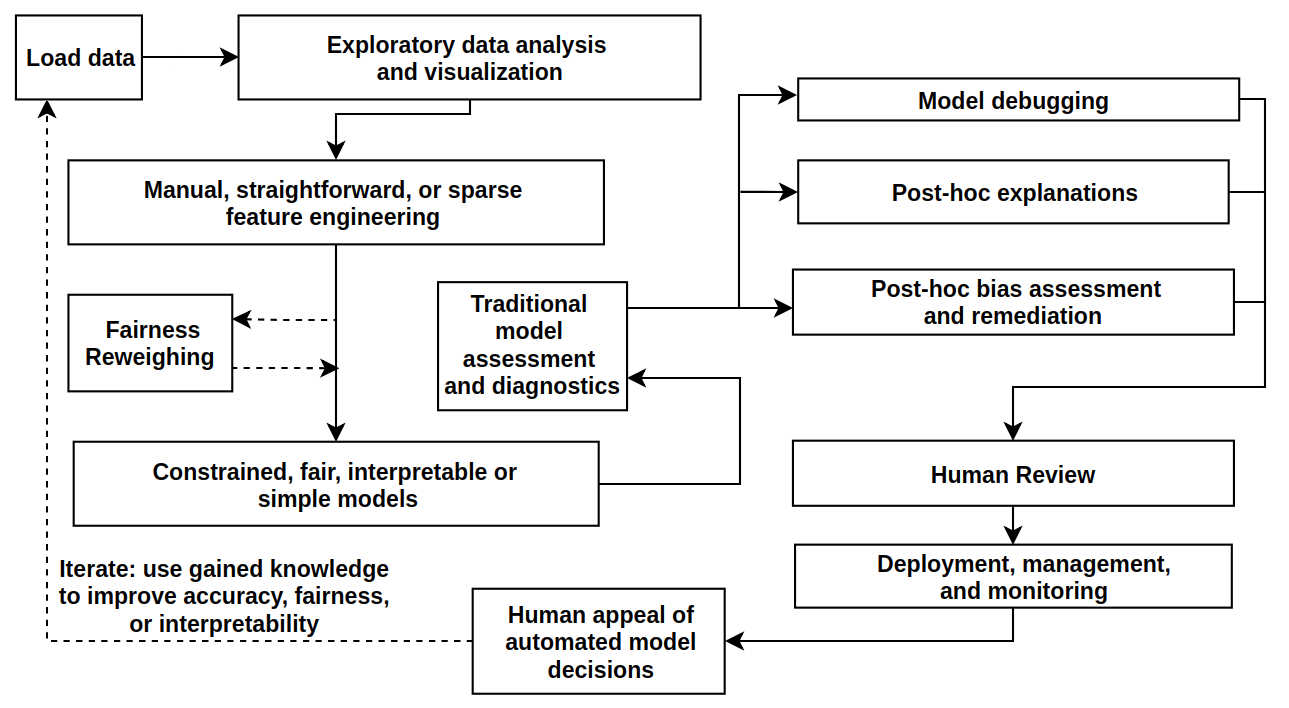
\includegraphics[height=140pt]{img/blueprint.png}
					\label{fig:blueprint}
				\end{center}
			\end{figure}		
		
		\end{frame}


%-------------------------------------------------------------------------------
	\section{EDA}
%-------------------------------------------------------------------------------
	
		\begin{frame}
		
			\frametitle{EDA and Data Visualization}		
			
			\begin{columns}
	
				\column{0.5\linewidth}
				\centering
				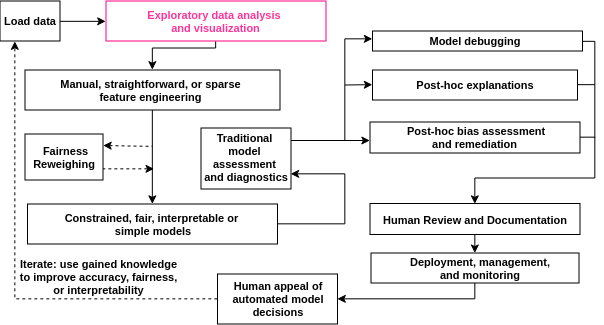
\includegraphics[height=100pt]{img/eda.png}
				
				\column{0.5\linewidth}
				\vspace{-5pt}
				\begin{itemize}
					\item Implemented in Driverless AI as AutoViz
					\item OSS: \href{https://ggplot2.tidyverse.org/}{ggplot}, \href{https://seaborn.pydata.org/}{seaborn}, etc.
					\item Reference: \textit{The Grammar of Graphics}, \cite{wilkinson2006grammar}
				\end{itemize}
				
			\end{columns}
		
		\end{frame}

%-------------------------------------------------------------------------------
	\section{Training}
%-------------------------------------------------------------------------------
	
		\begin{frame}
		
			\frametitle{Manual, Straightforward, or Sparse Feature Engineering}		
		
			\begin{columns}
	
				\column{0.5\linewidth}
				\centering
				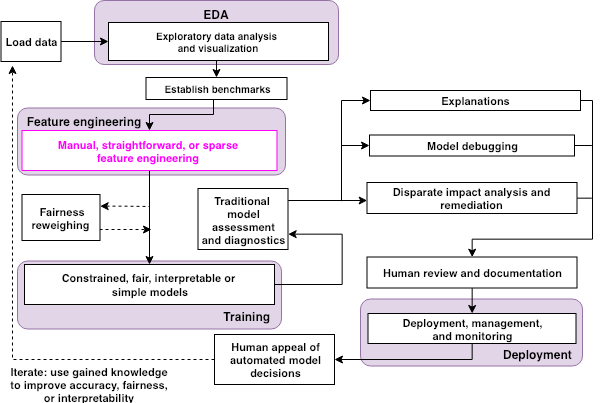
\includegraphics[height=100pt]{img/fe.png}
				
				\column{0.5\linewidth}
				\vspace{-5pt}
				\begin{itemize}
					\item Implemented in Driverless AI as high-interpretability transformers: frequency, interactions, (monotonic) weight-of-evidence, lags, basics and some Easter eggs in H2O-3
					\item Decades of custom coding in Hadoop, Python, R, SAS, Spark, SQL, etc.
					\item \href{https://github.com/szilard/benchm-databases}{Open benchmark of common tools}
				\end{itemize}
				
			\end{columns}		
		
		\end{frame}
	
		\begin{frame}
		
			\frametitle{Fairness Reweighing}		
			
			\begin{columns}
	
				\column{0.5\linewidth}
				\centering
				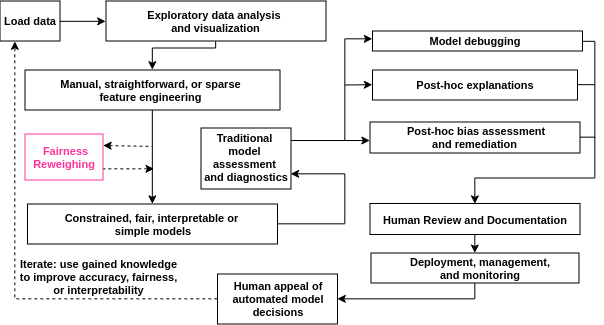
\includegraphics[height=100pt]{img/fr.png}
				
				\column{0.5\linewidth}
				\vspace{-5pt}
				\begin{itemize}
					\item Newer techniques for reweighing data prior to training to remove disparate impact analysis.
					\item OSS: IBM \href{https://github.com/IBM/AIF360}{AI360}
					\item References: \cite{calders2010three}, \cite{kamiran2012data},\cite{feldman2015certifying}, \cite{calmon2017optimized}
					\item \textcolor{magenta}{Roamap items for MLI-2}
				\end{itemize}
				
			\end{columns}			
			
		\end{frame}

		\begin{frame}
		
			\frametitle{Constrained, Fair, Interpretable or Simple Models}		
			
			\begin{columns}
	
				\column{0.5\linewidth}
				\centering
				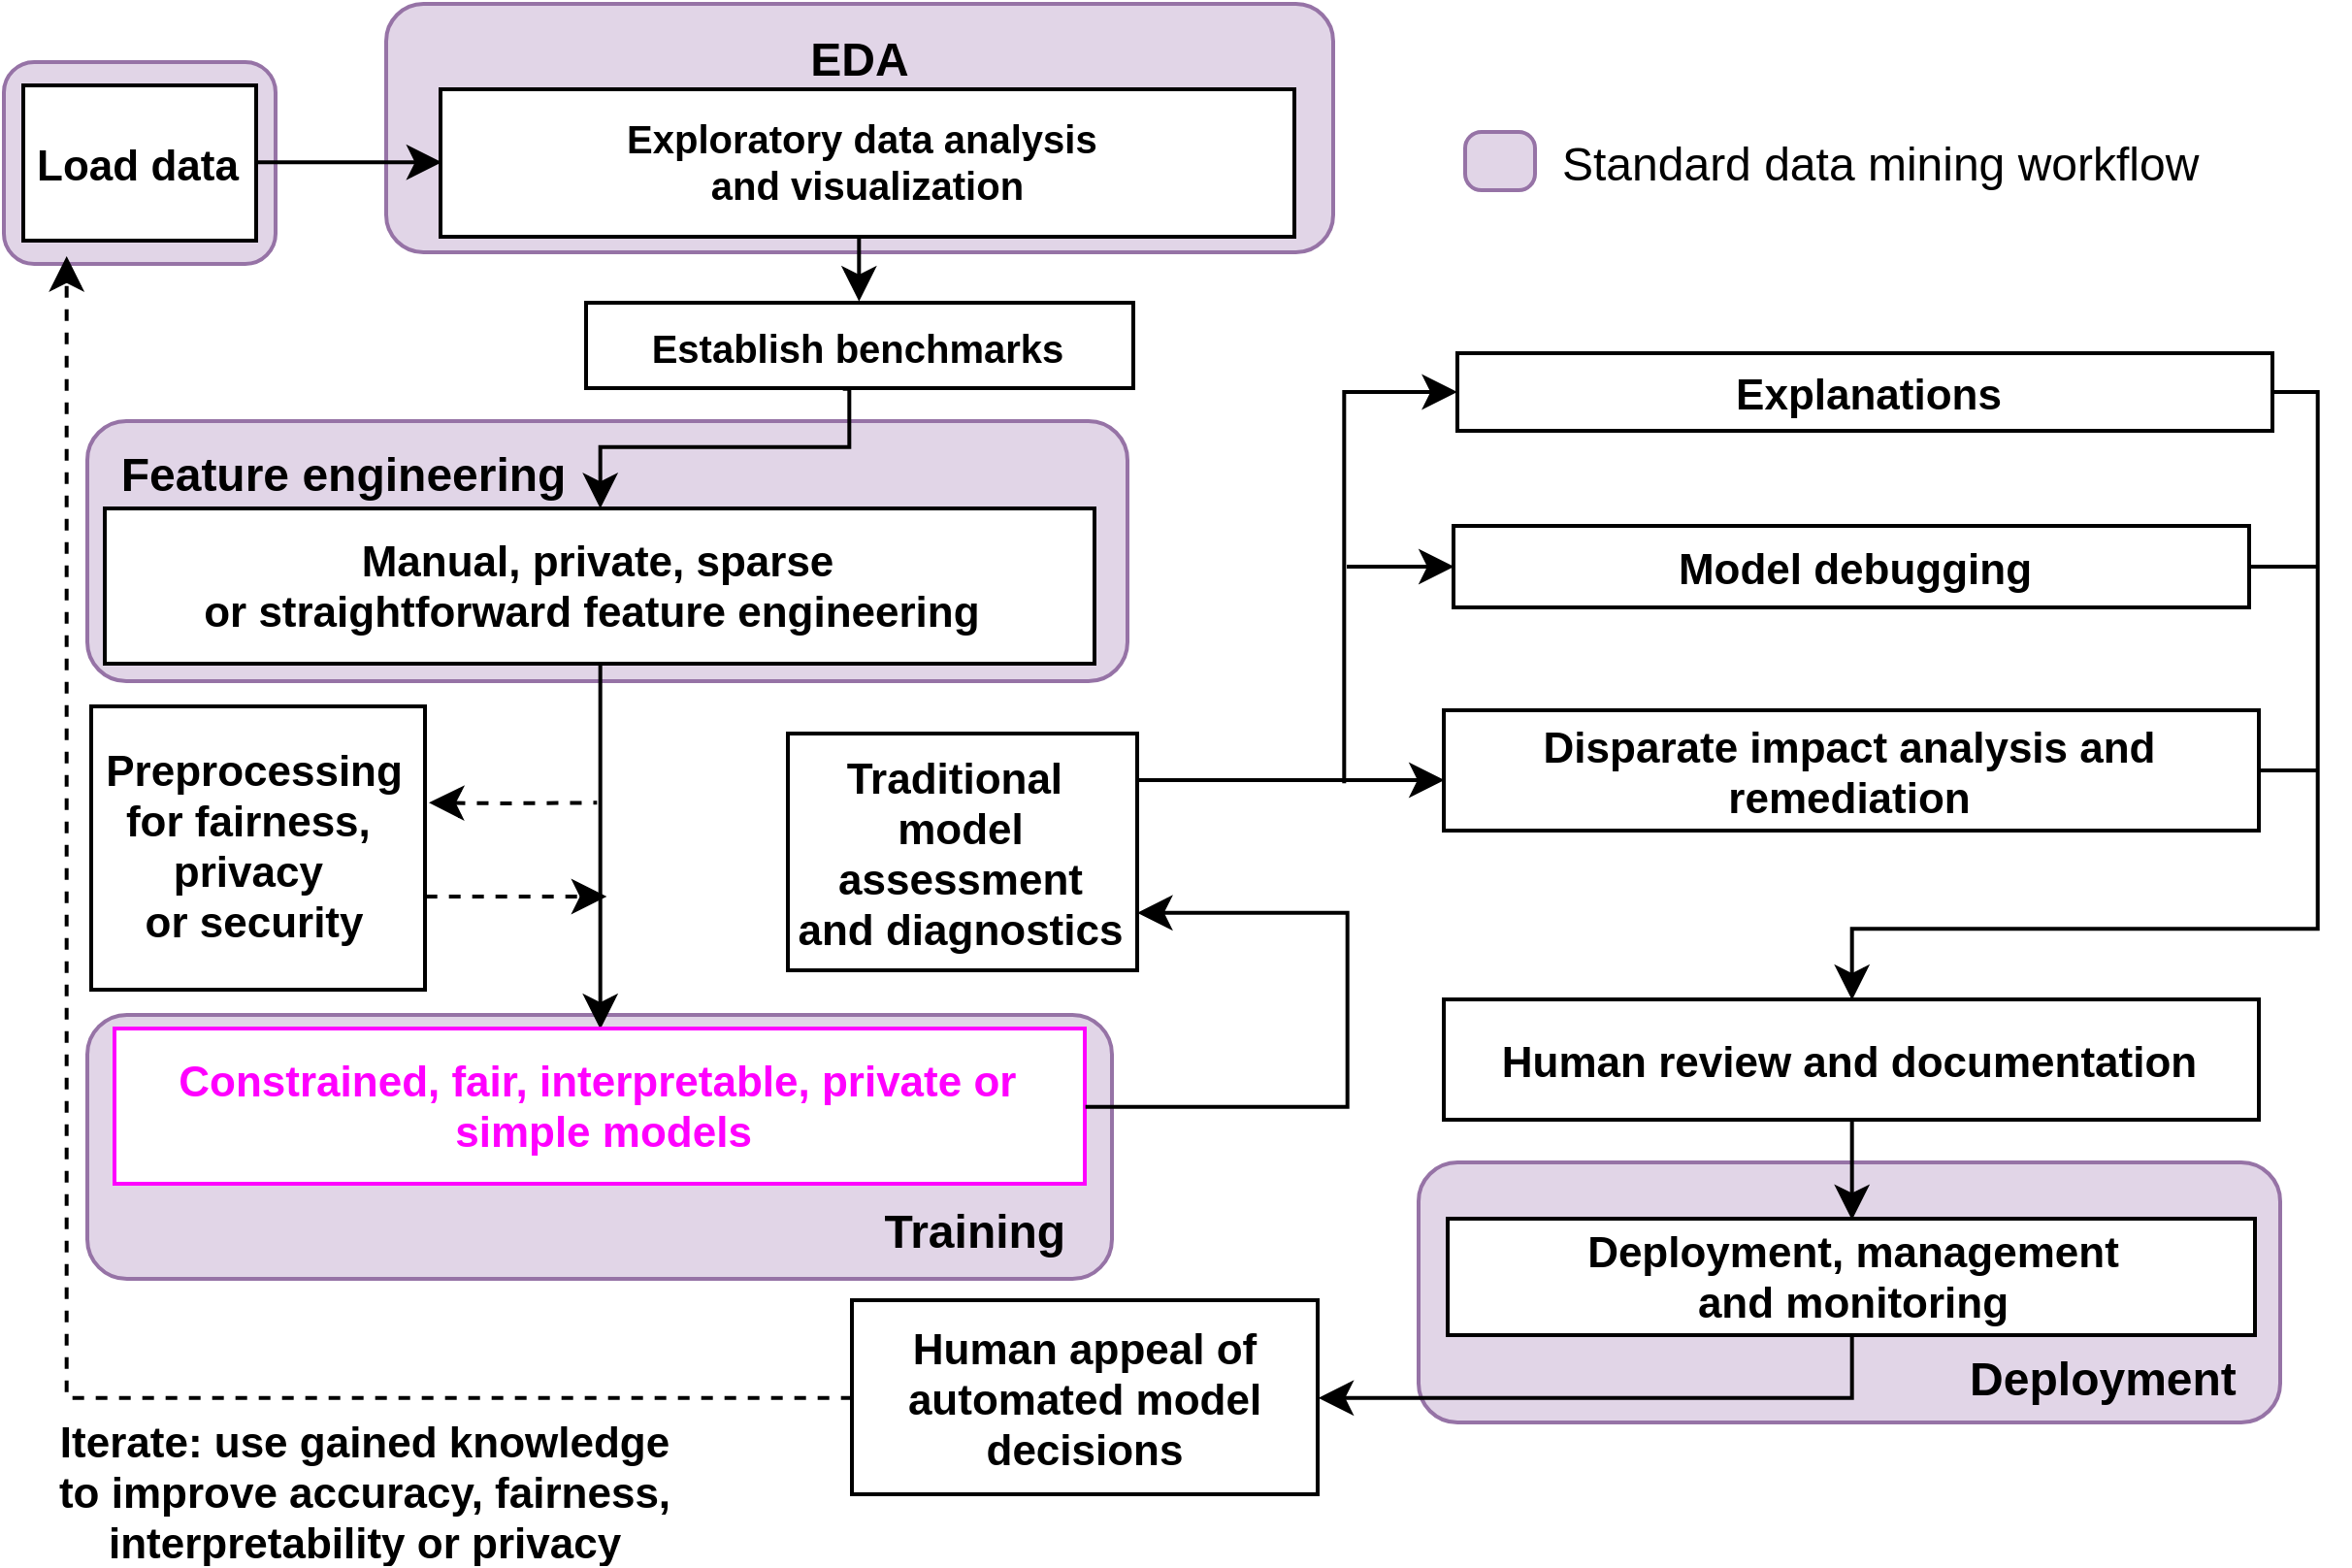
\includegraphics[height=100pt]{img/im.png}
				
				\column{0.5\linewidth}
				\vspace{-5pt}
				\begin{itemize}
					\item For best transparency use constrained, simple, or directly interpretable models from the beginning
					\item Implemented in Driverless AI as GLM, RuleFit, Monotonic GBM, in H2O-3 as GLM, monotonic GBM
					\item \textcolor{magenta}{Decision tree, scalable Bayesian rulelist, XNN are roadmap items for MLI-2}
				\end{itemize}
				
			\end{columns}			
			
		\end{frame}

%-------------------------------------------------------------------------------
	\section{Post-Hoc Analysis}
%-------------------------------------------------------------------------------

		\begin{frame}
		
			\frametitle{Traditional Model Assessment and Diagnostics}		
			
			\begin{columns}			
			
				\column{0.5\linewidth}
				\centering
				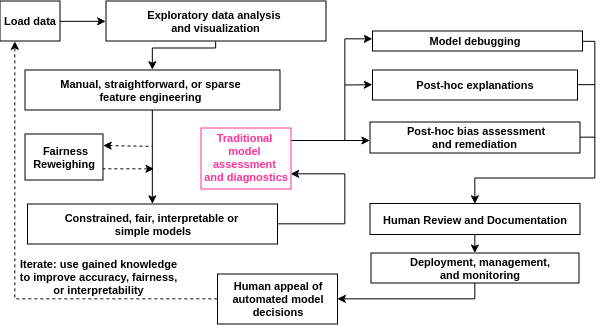
\includegraphics[height=100pt]{img/ma.png}
				
				\column{0.5\linewidth}
				\vspace{-5pt}
				\begin{itemize}
					\item Confirms model is accurate and meets assumption criteria
					\item Implemented as model diagnostics in Driverless AI
					\item Residual analysis is roadmap item for model diagnostics in Driverless AI
				\end{itemize}
				
			\end{columns}
		
		\end{frame}

		\begin{frame}
		
			\frametitle{Model Debugging}		
			
			\begin{columns}
	
				\column{0.5\linewidth}
				\centering
				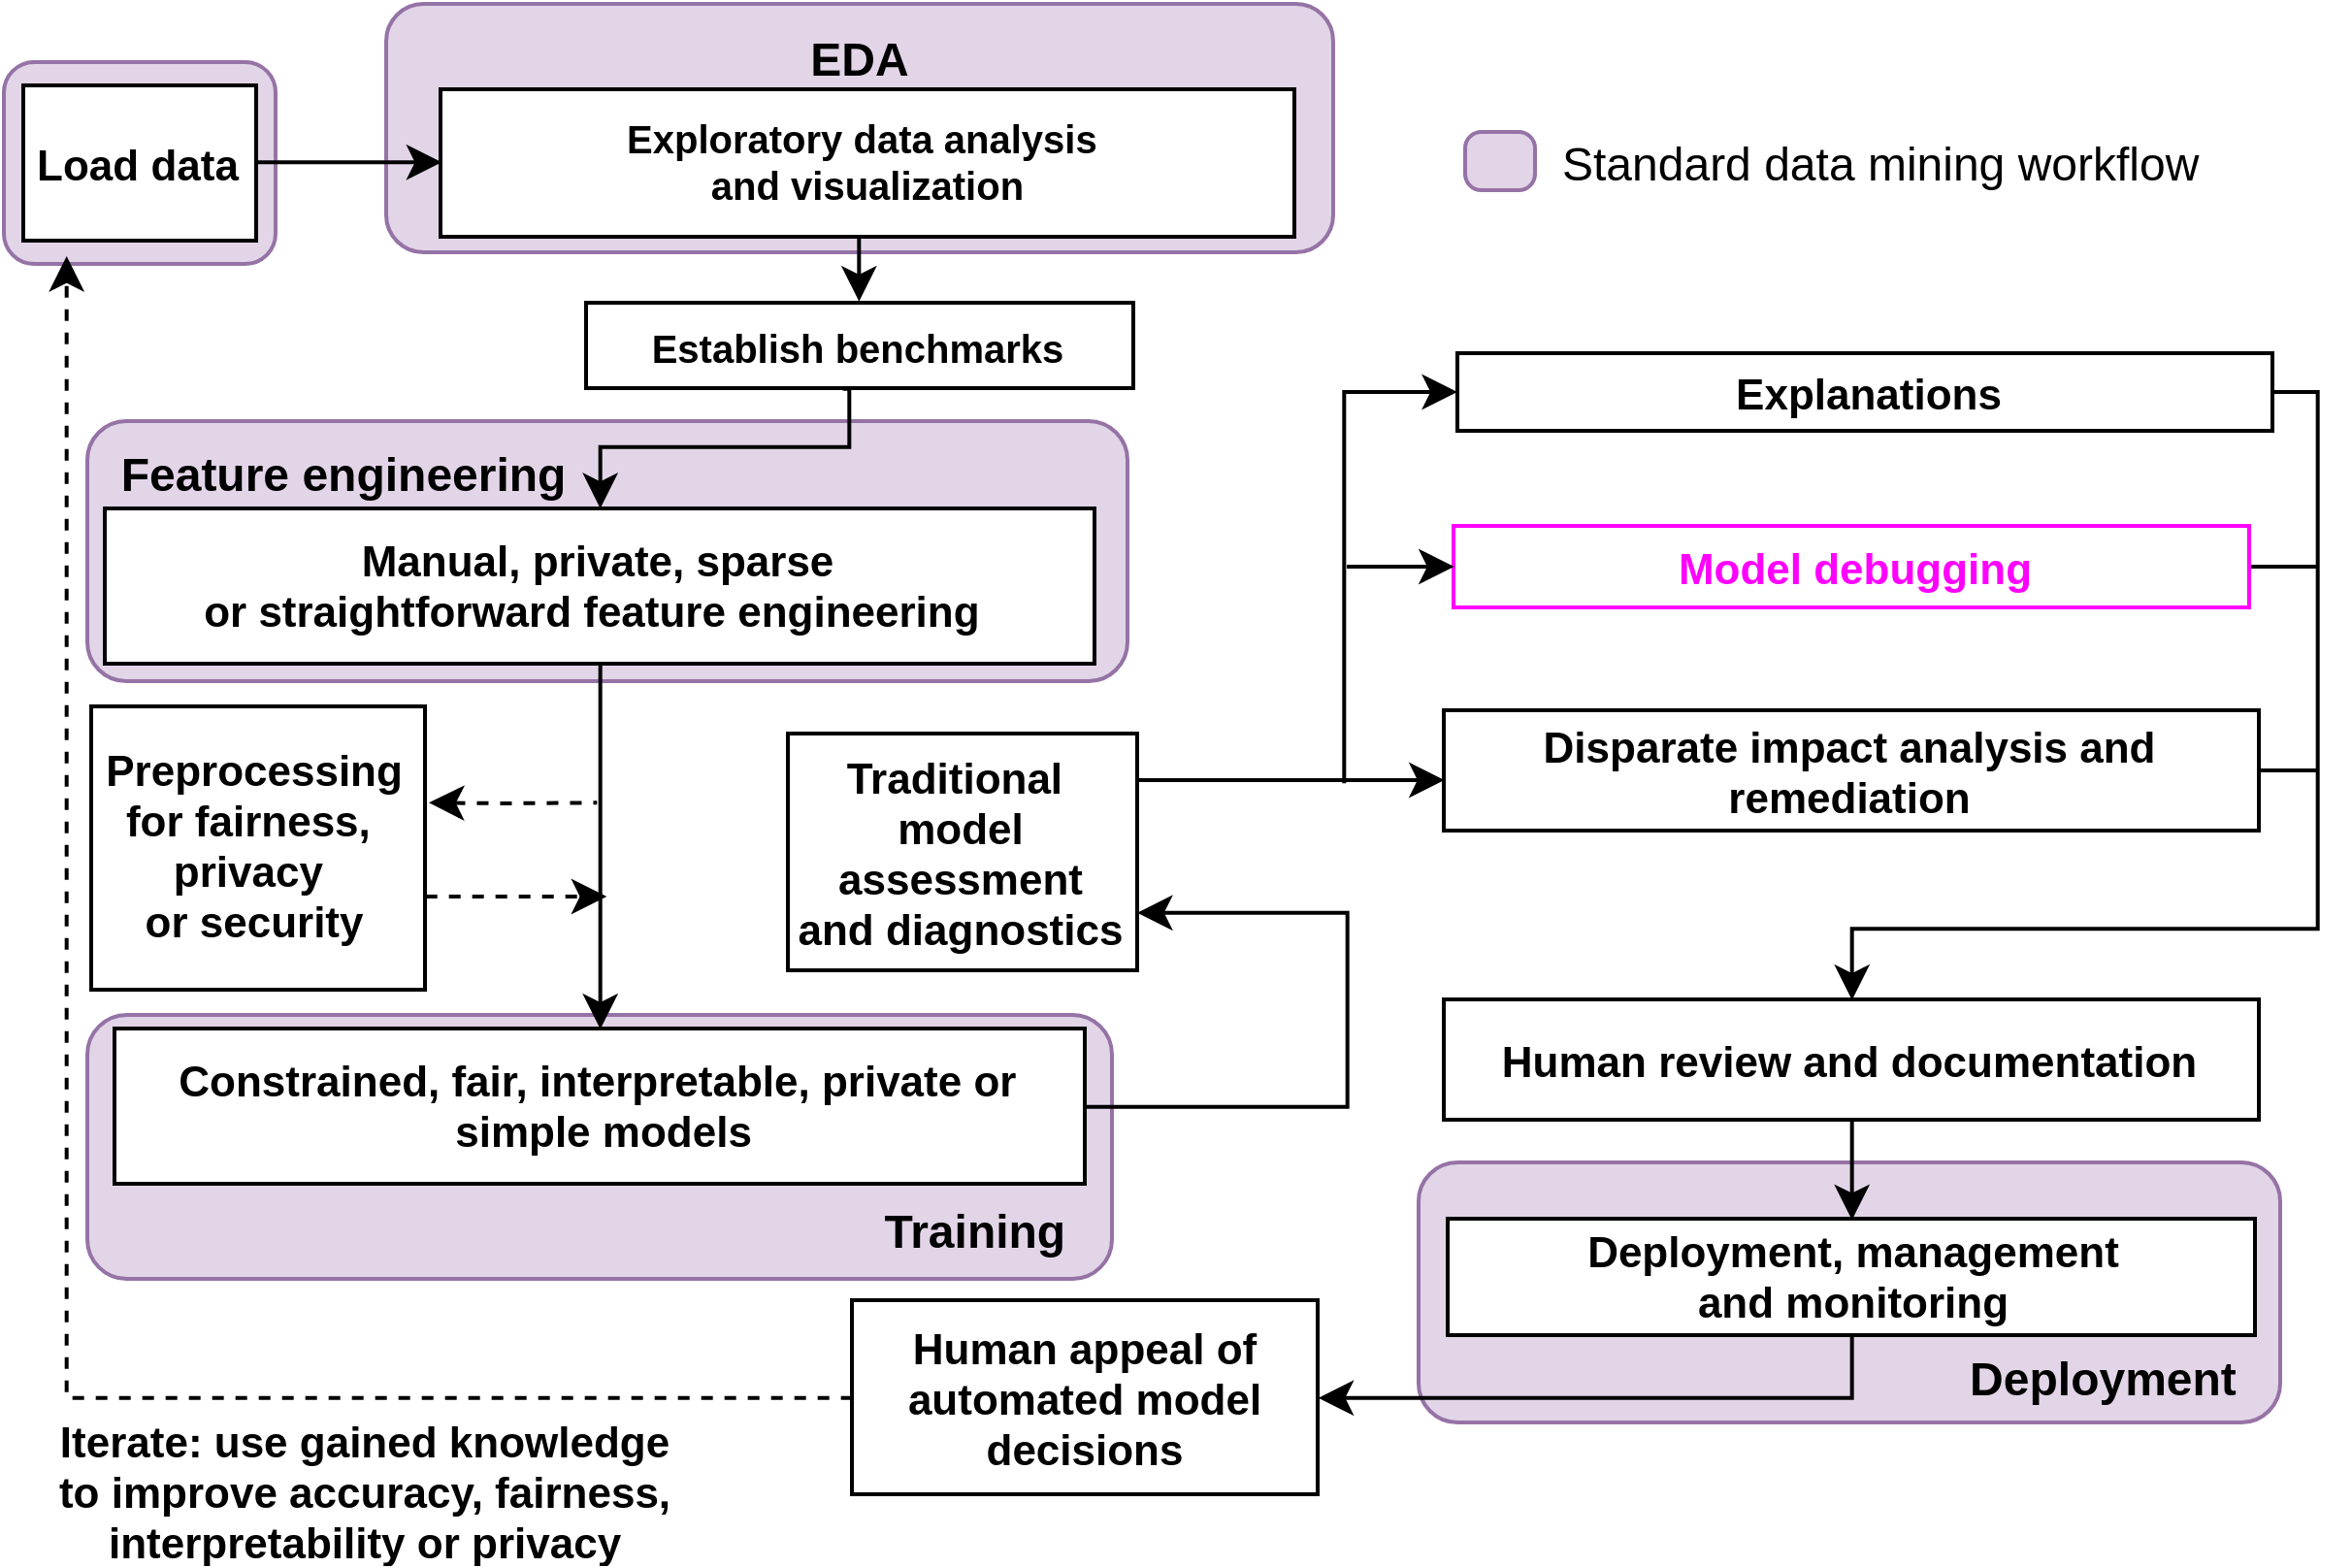
\includegraphics[height=100pt]{img/md.png}
				
				\column{0.5\linewidth}
				\vspace{-5pt}
				\begin{itemize}
					\item Newer techniques concerned with understanding and eliminating errors in model predictions; also model testing: "what-if" analysis, random attacks; focus on enhancing \textit{trust}
					\item \textcolor{magenta}{"what-if" analysis, explanation of residuals, measures of epistemic uncertainty are roadmap items for MLI-2}
				\end{itemize}
				
			\end{columns}			
		
		\end{frame}

		\begin{frame}
		
			\frametitle{Post-hoc Explanations}		
			
			\begin{columns}
	
				\column{0.5\linewidth}
				\centering
				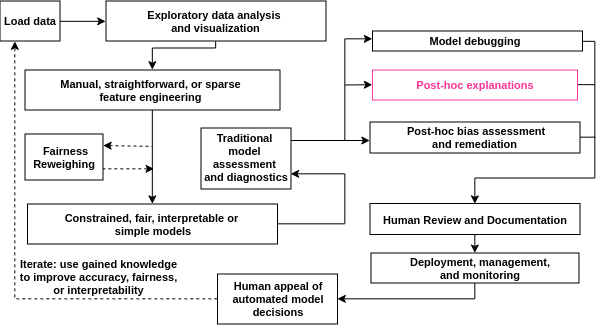
\includegraphics[height=100pt]{img/exp.png}
				
				\column{0.5\linewidth}
				\vspace{-5pt}
				\begin{itemize}
					\item Explanations enhance \textit{understanding}
					\item Global feature importance, surrogate decision tree, LIME, LOCO, treeinterpreter and Shapley local feature importance, partial dependence and ICE implemented in current MLI, Friedman's H-statistic implemented in MLI-2
					\item Shapley is roadmap item for H2O-3; \textcolor{magenta}{Basic term weights, ALE plots, decision boundary plots are roadmap items for MLI-2}
				\end{itemize}
				
			\end{columns}
		
		\end{frame}

		\begin{frame}
		
			\frametitle{Post-hoc Disparate Impact Assessment and Remediation}		
			
			\begin{columns}
	
				\column{0.5\linewidth}
				\centering
				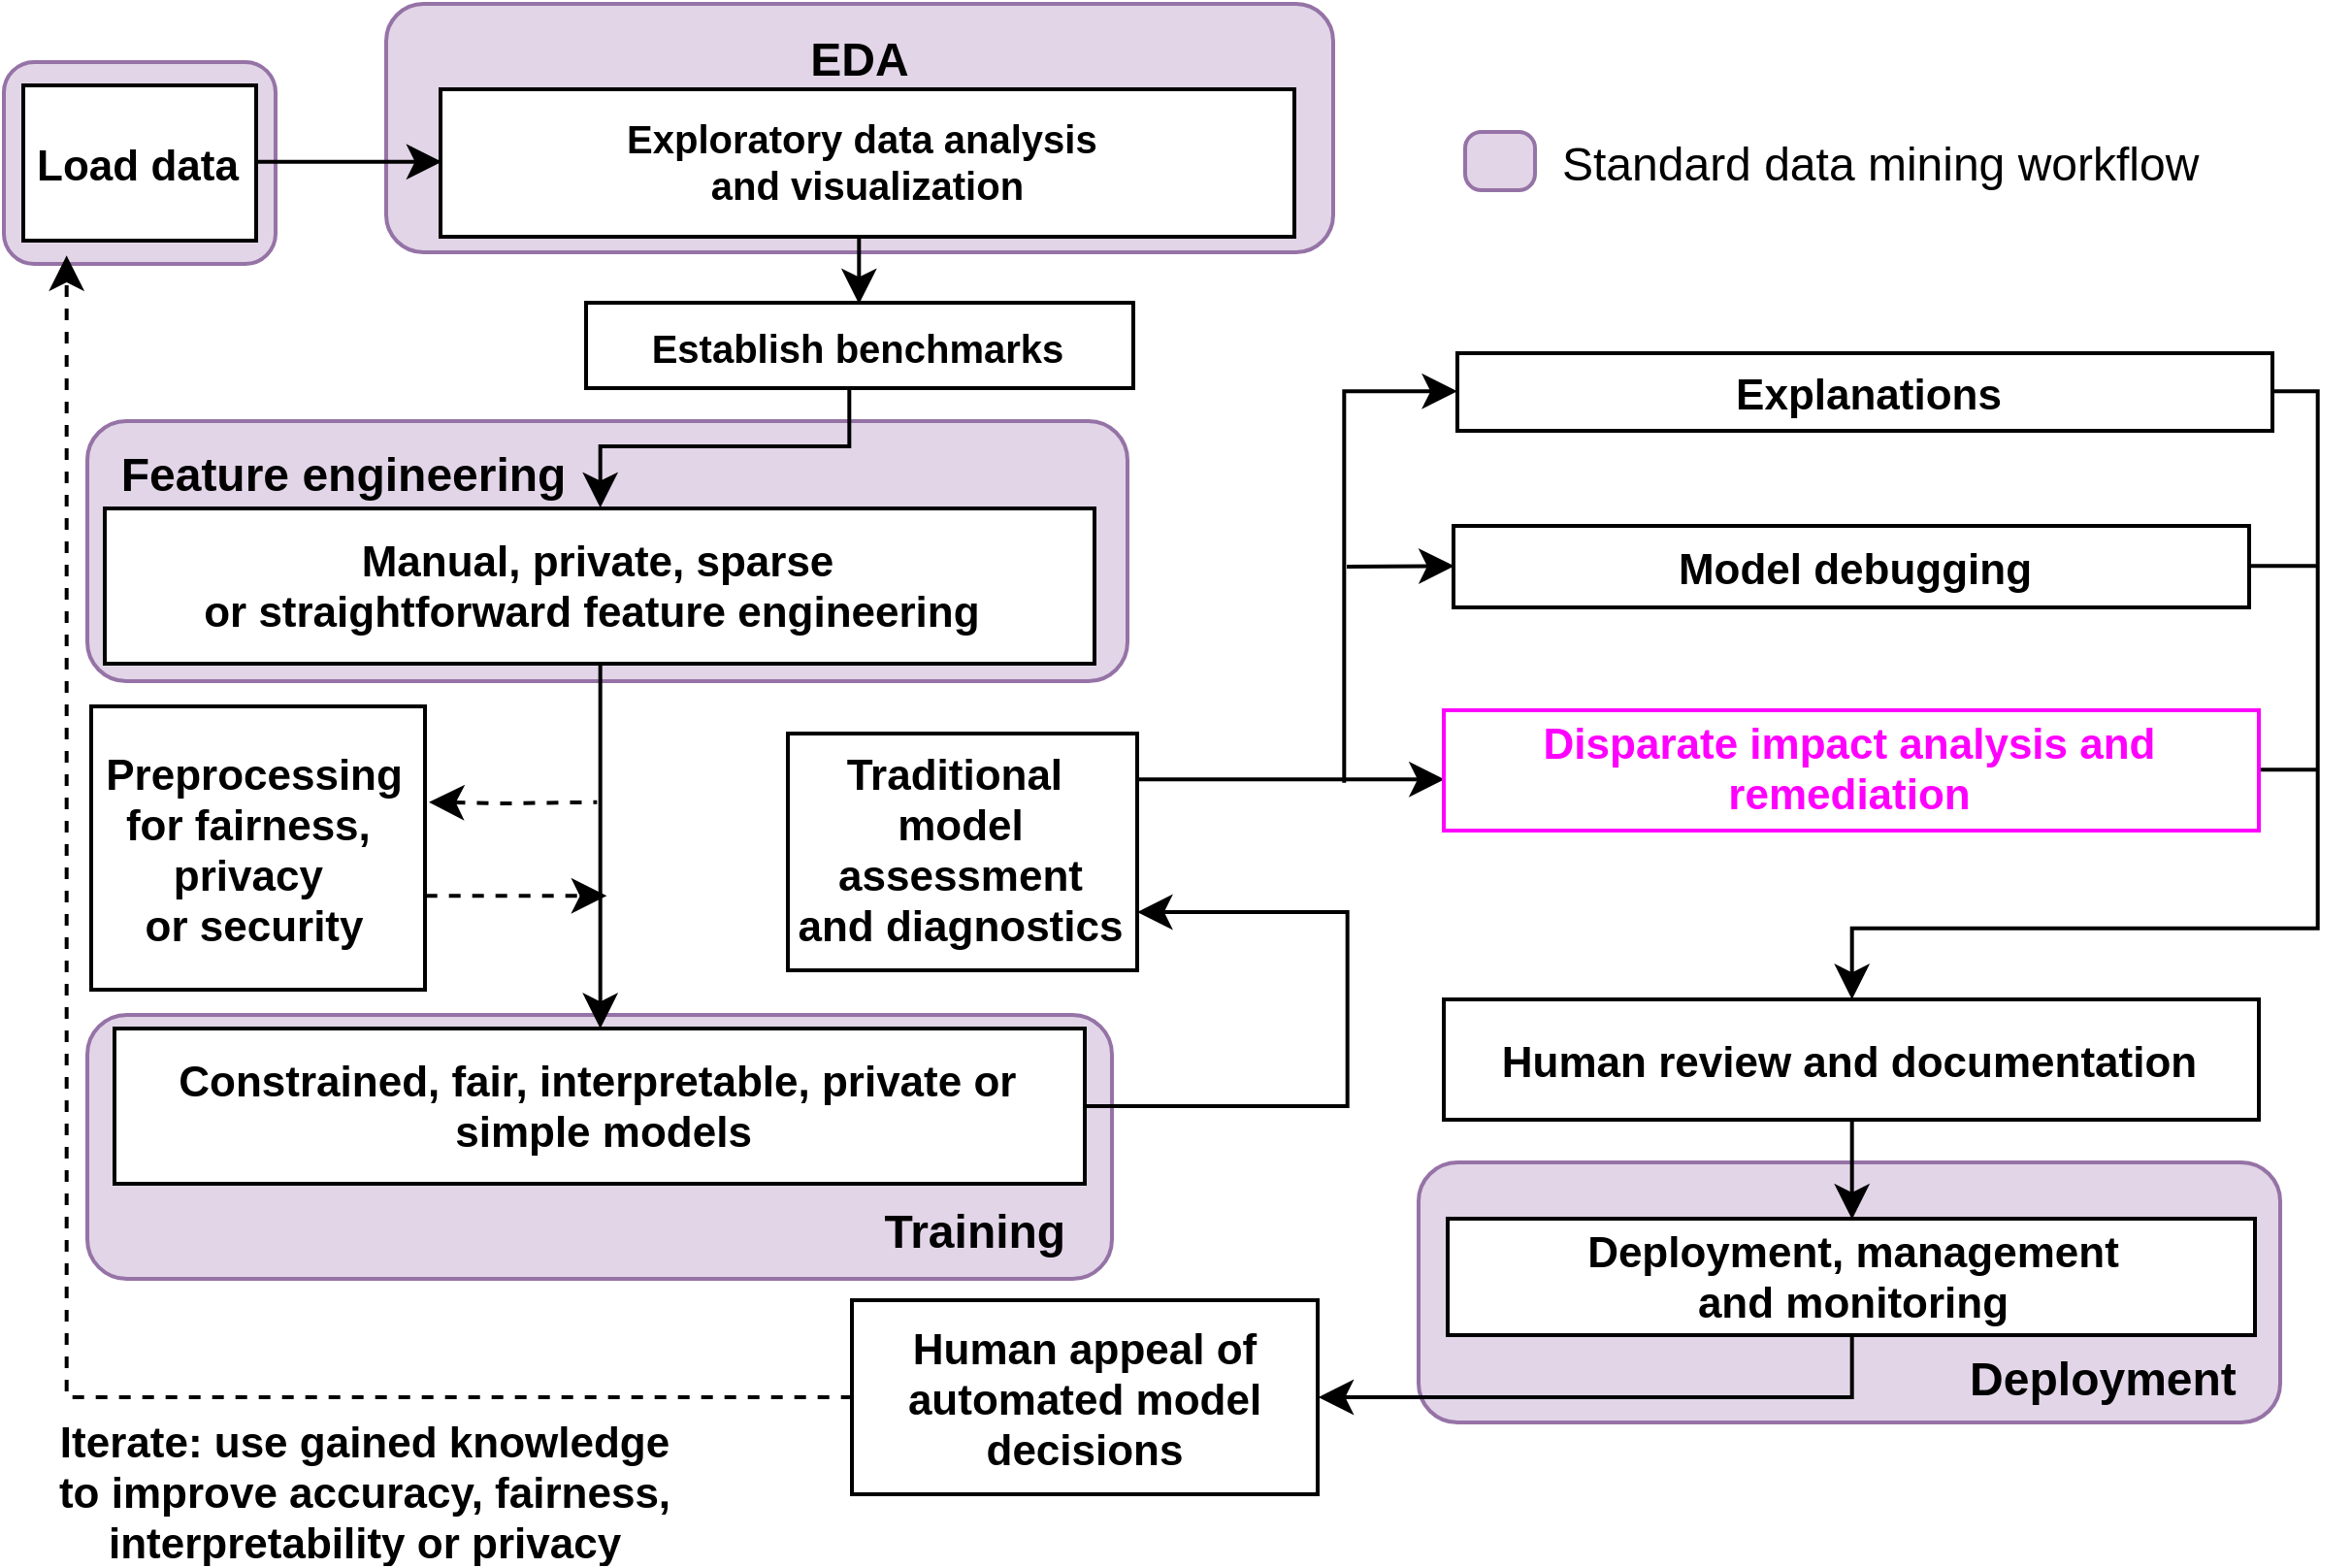
\includegraphics[height=100pt]{img/fair.png}
				
				\column{0.5\linewidth}
				\vspace{-5pt}
				\begin{itemize}
					\item Disparate Impact Analysis available through code APIs in Driverless AI and H2O-3
					\item Newer techniques can remove certain types of disparate impact 
					\item \textcolor{magenta}{Disparate impact remediation is a roadmap item for MLI-2}
				\end{itemize}
				
			\end{columns}
		
		\end{frame}

%-------------------------------------------------------------------------------
	\section{Human Review}
%-------------------------------------------------------------------------------

		\begin{frame}
		
			\frametitle{Human Review and Documentation}		
			
			\begin{columns}
	
				\column{0.5\linewidth}
				\centering
				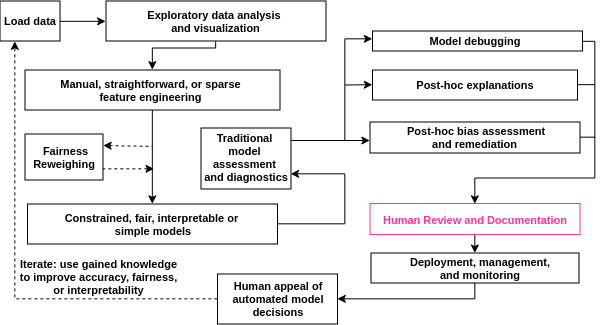
\includegraphics[height=100pt]{img/hr.png}
				
				\column{0.5\linewidth}
				\vspace{-5pt}
				\begin{itemize}
					\item Implemented as AutoDoc in\\ Driverless AI 
					\item Results from various roadmap items to be added to AutoDoc as appropriate
				\end{itemize}
				
			\end{columns}
		
		\end{frame}

%-------------------------------------------------------------------------------
	\section{Deployment}
%-------------------------------------------------------------------------------

		\begin{frame}

			\frametitle{Deployment, Management, and Monitoring}		
			
			\begin{columns}
	
				\column{0.4\linewidth}
				\centering
				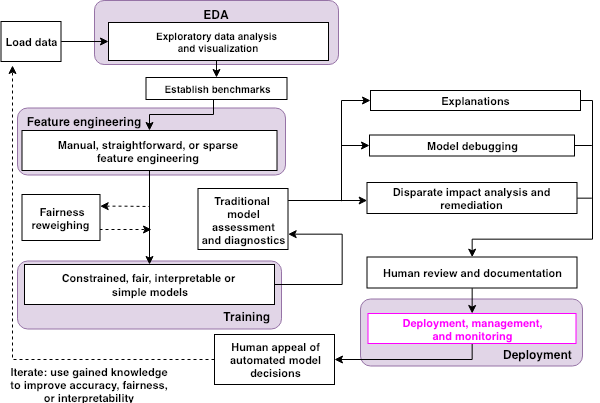
\includegraphics[height=100pt]{img/deploy.png}
				
				\column{0.5\linewidth}
				\vspace{-5pt}
				\begin{itemize}
					\item Monitor models for accuracy and fairness in real-time
					\item Broader roadmap item for H2O as a company
				\end{itemize}
				
			\end{columns}
		
		\end{frame}

%-------------------------------------------------------------------------------
	\section{Human Appeal}
%-------------------------------------------------------------------------------

		\begin{frame}	
			\frametitle{Iterate: Use Gained Knowledge to Improve Accuracy, Fairness, or Interpretability}		
			
			\begin{figure}[htb]
				\begin{center}
					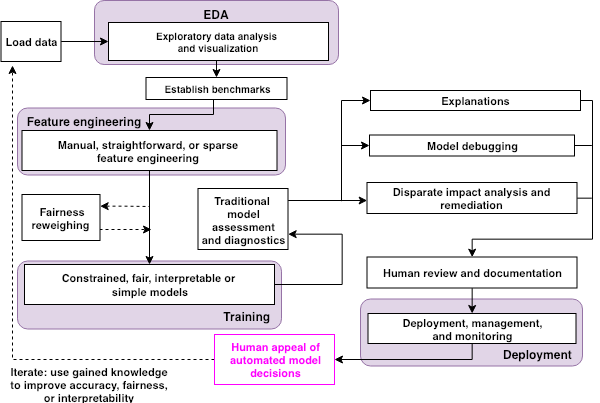
\includegraphics[height=120pt]{img/ha.png}
					\label{fig:blueprint}
				\end{center}
			\end{figure}	

			\centering
Very important, but probably requires custom implementation for each deployment

		\end{frame}

%-------------------------------------------------------------------------------
	\section{Iterate}
%-------------------------------------------------------------------------------

		\begin{frame}	

			\frametitle{Iterate: Use Gained Knowledge to Improve Accuracy, Fairness, or Interpretability}		
			
			\begin{figure}[htb]
				\begin{center}
					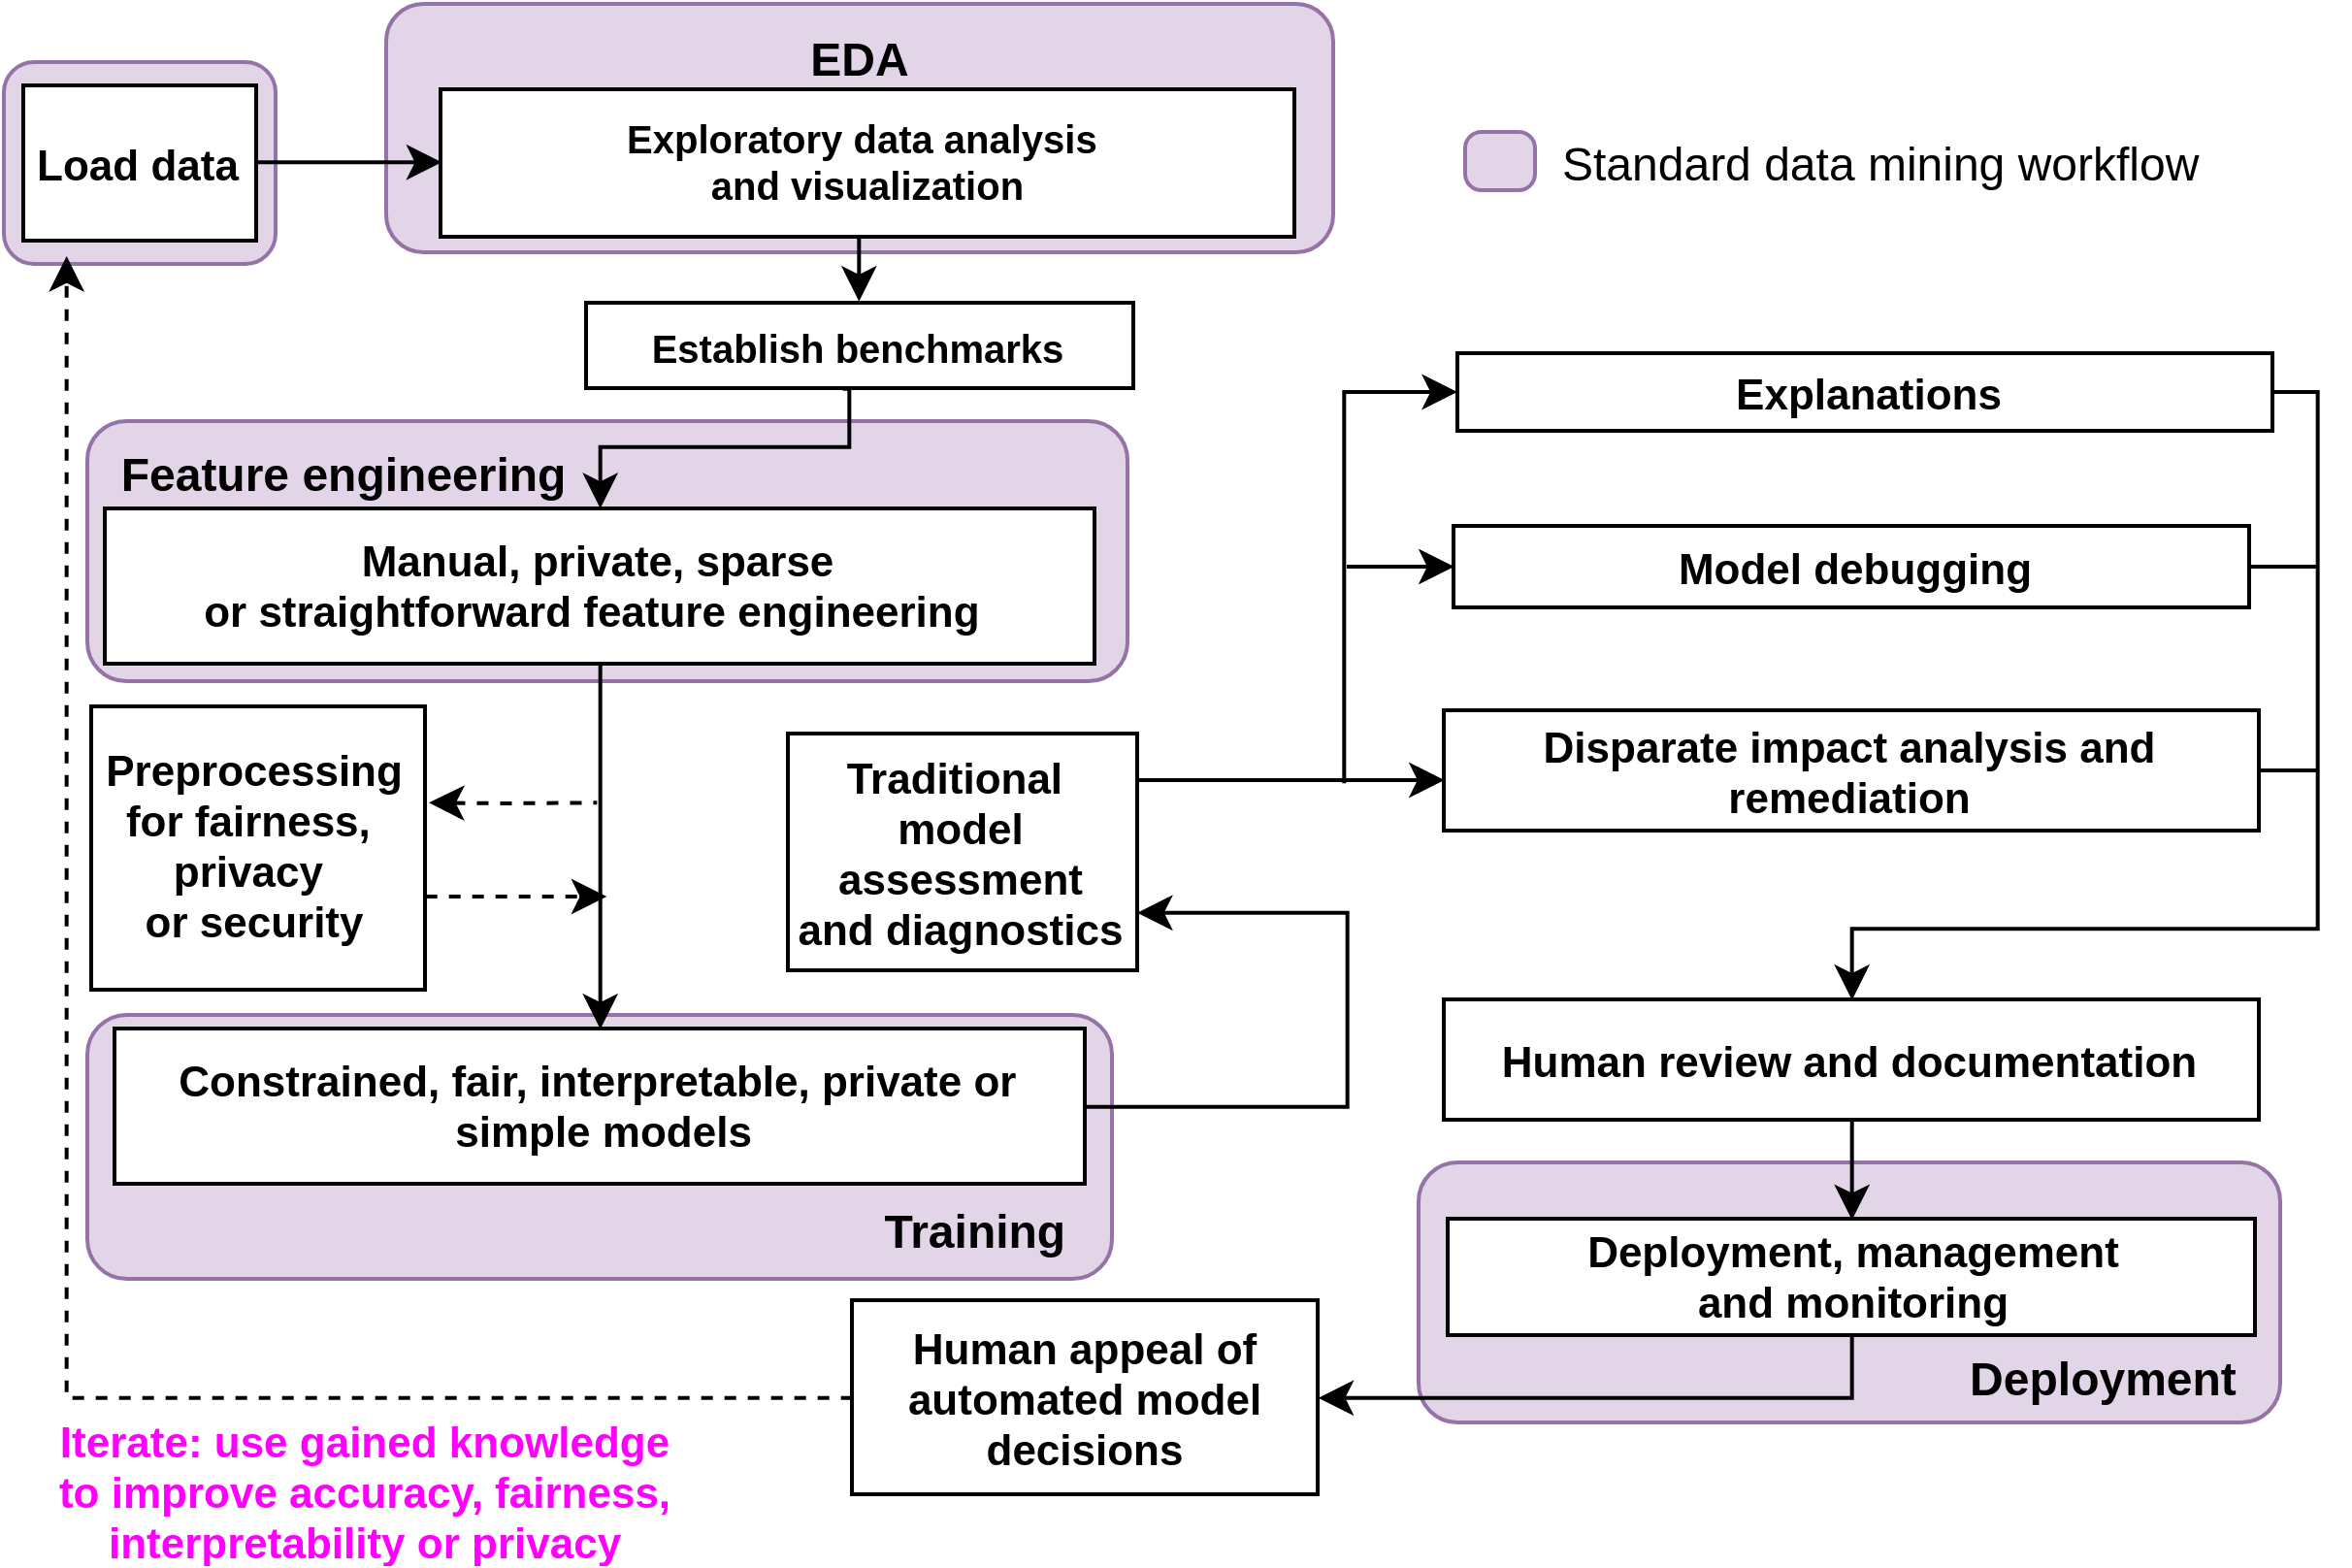
\includegraphics[height=120pt]{img/iter.png}
					\label{fig:blueprint}
				\end{center}
			\end{figure}	

			\centering
			Improvements, KPIs should not be restricted to accuracy alone
		
		\end{frame}

%-------------------------------------------------------------------------------
	\section{Open Questions}
%------------------------------------------------------------------------------

		\begin{frame}

			\frametitle{Open Questions}		

			\begin{itemize}
				\item What is the role for automation?
				\item How to implement human appeals, is it productizable?
			\end{itemize}
			
		\end{frame}

%-------------------------------------------------------------------------------
%	References
%-------------------------------------------------------------------------------


	\begin{frame}[t, allowframebreaks]
	
		\frametitle{References}
		
		\printbibliography
		
	\end{frame}

\end{document}